\section{Problem 2}
\label{sec:problem2}

The course notes (Section 5.6) state:
\begin{itemize}
  \item $1 < R < 11.94$: the Hohmann transfer is the minimum-impulse transfer.
  \item $R > 11.94$: the bi-parabolic transfer outperforms the Hohmann transfer.
  \item $R > 15.58$: any bi-elliptic transfer with $S > 1$ outperforms the Hohmann transfer.
\end{itemize}

\noindent Using the normalized impulse expressions from Problem 1, \texttt{problem2.py} uses the \texttt{scipy} root-finder \texttt{brentq} to solve the following root-finding problems.

\subsection*{(a) Hohmann vs. bi-parabolic}

The total impulse of each transfer is the sum of its impulses. Summing \eqref{eq:p1-hohmann} and \eqref{eq:p1-biparabolic},
\begin{align*}
\frac{\Delta v_H}{v_{c1}} &= \frac{\Delta v_{1,H}}{v_{c1}} + \frac{\Delta v_{2,H}}{v_{c1}}
  = \sqrt{\frac{2R}{1+R}} - 1 + \sqrt{\frac{1}{R}} - \sqrt{\frac{2}{R(1+R)}}\\[4pt]
\frac{\Delta v_{BP}}{v_{c1}} &= \frac{\Delta v_{1,BP}}{v_{c1}} + \frac{\Delta v_{2,BP}}{v_{c1}}
  = \left(\sqrt{2}-1\right)\left(1+\sqrt{\frac{1}{R}}\right)
\end{align*}
The crossover is the value of $R$ at which the two totals are equal, i.e.\ the root of
\begin{equation}
\boxed{f(R) = \frac{\Delta v_H}{v_{c1}} - \frac{\Delta v_{BP}}{v_{c1}} = 0}
\label{eq:p2-fbp}
\end{equation}
solved with \texttt{brentq} on the bracket $R\in[2,50]$, over which $f$ changes sign.

\subsection*{(b) Hohmann vs. bi-elliptic, for each $S$}

Summing the three impulses of \eqref{eq:p1-bielliptic},
\begin{equation*}
\frac{\Delta v_{BE}}{v_{c1}} = \sqrt{\frac{2RS}{1+RS}} - 1
+ \sqrt{\frac{1}{RS}}\left(\sqrt{\frac{2}{1+S}} - \sqrt{\frac{2}{1+RS}}\right)
+ \sqrt{\frac{2S}{R+RS}} - \sqrt{\frac{1}{R}}
\end{equation*}
For each $S\in\{2,5,10,11,12,15\}$, the crossover is the root of
\begin{equation}
\boxed{g(R;S) = \frac{\Delta v_H}{v_{c1}} - \frac{\Delta v_{BE}}{v_{c1}} = 0}
\label{eq:p2-fbe}
\end{equation}
where $\Delta v_H/v_{c1}$ is the same Hohmann total impulse as shown in part (a). Each root is solved with \texttt{brentq} on the bracket $R\in[2,50]$.

\medskip
\programoutput{outputs/problem2.txt}

\subsection*{(c) Root as a function of $S$}

\begin{figure}[H]
\centering
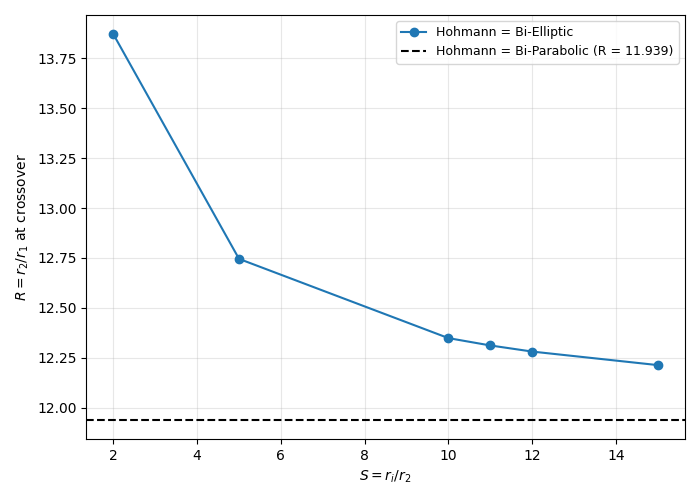
\includegraphics[width=0.75\textwidth]{problem2_roots.png}
\caption{Hohmann/bi-elliptic crossover $R$ vs.\ $S$.}
\label{fig:p2-roots}
\end{figure}

\FloatBarrier
